\documentclass[14pt]{extarticle} 
\usepackage{amsmath,mathtools,amsfonts,amsthm,amssymb,hyperref,tikz}
\usepackage{wasysym,geometry,bussproofs,latexsym,parskip,bookmark}
\newtheorem{defn}{Definition}
\newtheorem{thm}{Theorem}
\newtheorem{claim}{Claim}
\newtheorem{lemma}{Lemma}
\hypersetup{colorlinks,allcolors=blue,linktoc=all}
\geometry{a4paper} 
\geometry{margin=0.5in}
\title{Math for CS 2015/2019 Midterm 3 solutions}
\author{https://github.com/spamegg1}
\begin{document}
\maketitle
\tableofcontents

\section{Problem 1 (Scheduling)}
The following DAG describes the prerequisites among tasks $\{A, \ldots, H \}$.

$A \to D$,

$B \to E, B \to F$,

$C \to F$,

$D \to E$, 

$E \to G$,

$F \to H$.
\subsection{(a)}
What are the two maximum size antichains?
\begin{proof}
A, D, E, G are all comparable to each other. Any antichain can only contain one of these.

B, E, G are all comparable to each other. Any antichain can only contain one of these.

B, F, H are all comparable to each other. Any antichain can only contain one of these.

C, F, H are all comparable to each other. Any antichain can only contain one of these.

So the maximum size of an antichain is 3. Also notice that any antichain of size 3 must include C.

Any antichain of size 3 includes C, so it cannot include F, H. So it must include B, so it cannot include E, G. So it must include A or D.

The only 2 antichains of size 3 are: A,B,C and D,B,C.
\end{proof}

\subsection{(b)}
If each task takes unit time to complete, what is the minimum parallel time to complete all the tasks?
\begin{proof}
The largest chain is $A \to D \to E \to G$, which has length 4. This is the critical path, so the minimum parallel time to complete all tasks is 4 units.
\end{proof}

\subsection{(c)}
What is the minimum parallel time if no more than two tasks can be completed in parallel?
\begin{proof}
This is still 4. A,C can be completed in parallel in 1 unit time. Then B,D can be completed in parallel in 1 unit time. Then E,F, and then G,H.
\end{proof}

\section{Problem 2 (Partial Orders \& Equivalence)}
Let $A$ be a nonempty set.
\subsection{(a)}
Describe a single relation on $A$ that is both an equivalence relation and a weak partial order on $A$.
\begin{proof}
Remember that equivalence means: reflexive, symmetric, transitive.

Weak partial order means: reflexive, antisymmetric, transitive.

The equality relation $R(a,b) \Coloneqq a = b$ on A satisfies all these: 

It is reflexive because $a = a$ for all $a \in A$.

It is symmetric because for all $a,b \in A$, if $a = b$ then $b = a$.

It is transitive because for all $a,b,c \in A$ if $a = b$ and $b = c$ then $a = c$.

It is antisymmetric because there are no $a \neq b \in A$ such that $R(a,b)$, so the definition ``$a \, R \, b$ IMPLIES NOT$(b \, R \, a)$'' is vacuously true.
\end{proof}

\subsection{(b)}
Prove that the relation of part (a) is the only relation on A with these properties.
\begin{proof}
Just to clarify, the relation $R$ from part (a) contains only the ``diagonal'' of $A \times A$:
$$
R = \{\langle a, a\rangle \,\, | \,\, a \in A\}
$$
We want to prove that if any other binary relation $S$ has the same properties then $S$ equals the above set.

1. Assume $S \subseteq A \times A$ is reflexive, symmetric, antisymmetric, and transitive.

2. Since $S$ is reflexive, $S$ contains $\langle a,a \rangle$ for all $a \in A$.

3. Now assume $a, b \in A$, $a \neq b$ and $\langle a,b \rangle \in S$. Then since $S$ is symmetric, $\langle b,a \rangle \in S$. But since $S$ is antisymmetric, $\langle b,a \rangle \notin S$, a contradiction.

4. Therefore for all $a, b \in A$ such that $a \neq b$, $S$ cannot contain $\langle a,b \rangle$.

5. Therefore by (2) and (4)
$$
S = \{\langle a, a\rangle \,\, | \,\, a \in A\}
$$
so $S$ is the same relation as $R$ from part (a).
\end{proof}

\section{Problem 3 (Simple Graphs)}
\subsection{(a)}
Give an example of a simple graph that has two vertices $u \neq v$ and two distinct paths between $u$ and $v$, but no cycle including either $u$ or $v$.

Hint: There is an example with 5 vertices.
\begin{proof}
Proof by picture:
\begin{center}
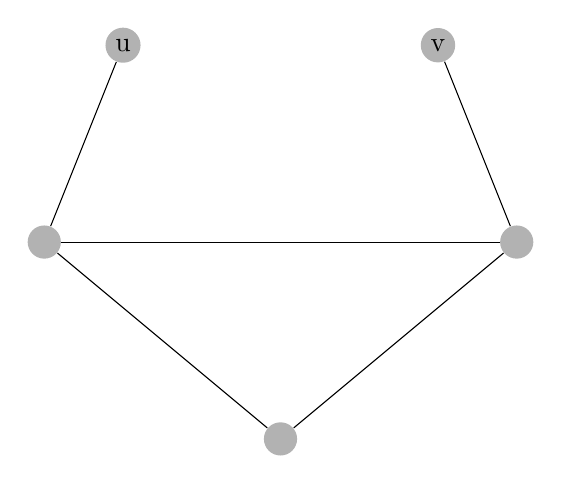
\begin{tikzpicture}
\tikzstyle{vertex}=[circle,fill=black!30,minimum size=12pt,inner sep=2pt]
\node[vertex] (G_1) at (2,2)    {v};
\node[vertex] (G_2) at (3,-0.5) {};
\node[vertex] (G_3) at (0,-3)   {};
\node[vertex] (G_4) at (-3,-0.5){};
\node[vertex] (G_5) at (-2,2)   {u};
\draw (G_1) -- (G_2) -- (G_3) -- (G_4) -- (G_5);
\draw (G_2) -- (G_4);
\end{tikzpicture}
\end{center}
\end{proof}

\subsection{(b)}
Prove that if there are different paths between two vertices in a simple graph, then the graph has a cycle.
\begin{proof}
1. Assume $u \neq v$ are vertices in a graph and $p \neq q$ are different paths between them. Let's explicitly write down $p, q$. There exist nodes $p_i$ and $q_j$, edges $e_i$ and $f_j$ such that:
$$
p: u = p_0 - e_0 - p_1 - e_1 - \ldots - p_{m-1} - e_m - p_m = v
$$
$$
q: u = q_0 - f_0 - q_1 - f_1 - \ldots - q_{n-1} - f_n - q_n = v
$$
2. If $p$ and $q$ have no nodes in common (except $u$ and $v$), then traversing $p$ followed by traversing $q$ backwards gives us the cycle:
$$
u = p_0 - e_0 - \ldots - e_m - p_m = v = q_n - f_n - \ldots - f_0 - q_0 = u
$$
3. So assume that $p$ and $q$ have a node in common (except $u$ and $v$). Say $k \geq 1$ is the smallest with the property that $p_k = q_l$ for some $l$.

4. Assume $p$ and $q$ have exactly one node $p_k = q_l$ in common. If $k = 1$ (so that $p_k$ is connected to $u$) then following $p_k$ to $v$ along $p$, then following along $q$ back to $p_k$ gives us the cycle:
$$
p_k - e_k - \ldots - e_m - p_m = v = q_n - f_n - \ldots - f_l - q_l = p_k
$$
If instead $k > 1$ then similarly we can start from $u$, travel to $p_k$ and travel back to $u$ to get a cycle.

5. Otherwise $p$ and $q$ have at least two nodes in common. Say $k_1 < k_2$ are the two smallest with the property that $p_{k_1} = q_{l_1}$ and $p_{k_2} = q_{l_2}$ for some $l_1 < l_2$. 

Then, going from $p_{k_1}$ to $p_{k_2}$ along $p$, then going back from $p_{k_2}$ to $p_{k_1}$ along $q$ gives us the cycle:
$$
p_{k_1} - e_{k_1} - \ldots - e_{k_2} - p_{k_2} = q_{l_2} - f_{l_2} - \ldots - f_{l_1} - q_{l_1} = p_{k_1}
$$
\end{proof}

\section{Problem 4 (Trees \& Coloring)}
Prove by induction that, using a fixed set of $n > 1$ colors, there are exactly $n\cdot(n-1)^{m-1}$ different colorings of any tree with $m$ vertices.
\begin{proof}
We use induction on $m$, the number of vertices.

{\bf Base Case.} $m = 1$. There is only one vertex. There are $n$ colors. So there are $n$ different ways to color this one vertex. This agrees with the formula:
$$
n\cdot(n-1)^{m-1} = n\cdot(n-1)^{1-1} = n\cdot(n-1)^{0} = n \cdot 1 = n
$$

{\bf Induction Step.} Assume $m \geq 1$ and assume there are exactly $n\cdot(n-1)^{m-1}$ different colorings of any tree with $m$ vertices.

Now consider a tree $T$ with $m+1$ vertices (notice $m+1 \geq 2$). Consider a leaf $l$ of $T$. Then $l$ is connected to only one node of $T$, say $n$, with an edge, say $e$. 

Consider the smaller tree $T'$ obtained by removing $l$ and $e$ from $T$. This is still a tree because we only removed a leaf. Also notice that $T'$ has $m$ vertices. 

Now consider colorings of $T$. Every coloring of $T$ is obtained from a coloring of $T'$ plus a coloring of the leaf node $l$. Since $l$ is connected to $n$, $l$ cannot be colored with the same color as $n$. 

Therefore, given a coloring of $T'$, there are $n-1$ ways to color $l$ to obtain a coloring of $T$. By the induction hypothesis there are $n\cdot(n-1)^{m-1}$ different colorings of $T'$. So there are 
$$
n\cdot(n-1)^{m-1} \cdot (n-1) = n\cdot(n-1)^{m}
$$ 
different colorings of $T$. This completes the proof of the induction step. 

By the Principle of Mathematical Induction, there are exactly $n\cdot(n-1)^{m-1}$ different colorings of any tree with $m$ vertices.
\end{proof}

\section{Problem 5 (Stable Marriage)}
The Mating Ritual for finding stable marriages works without change when there are at least as many, and possibly more, men than women. You may assume this. So the Ritual ends with all the women married and
no rogue couples for these marriages, where an unmarried man and a married woman who prefers him to her spouse is also considered to be a ``rogue couple.''

Let Alice be one of the women, and Bob be one of the men. Circle the properties below that are preserved invariants of the Mating Ritual when there are at least as many men as women.
\subsection{(a)}
Alice has a suitor (man who is serenading her) whom she prefers to Bob.
\begin{proof}
\end{proof}

\subsection{(b)}
Alice is the only woman on Bob's list.
\begin{proof}
\end{proof}

\subsection{(c)}
Alice has no suitor.
\begin{proof}
\end{proof}

\subsection{(d)}
Bob prefers Alice to the women he is serenading.
\begin{proof}
\end{proof}

\subsection{(e)}
Bob is serenading Alice.
\begin{proof}
\end{proof}

\subsection{(f)}
Bob is not serenading Alice.
\begin{proof}
\end{proof}

\subsection{(g)}
Bob's list of women to serenade is empty.
\begin{proof}
\end{proof}

\section{Problem 6 (Sums \& Integrals)}
There is a number $a$ such that
$$
\sum_{i=1}^{\infty}i^p
$$
converges to a finite value iff $p < a$.
\subsection{(a)}
What is the value of $a$?
\begin{proof}
$a = -1$.
\end{proof}

\subsection{(b)}
Circle all of the following that would be good approaches as part of a proof that this value of $a$ is correct.

{\bf (i)} Find a closed form for
$$
\int_1^{\infty}x^p\,dx
$$
\begin{proof}
Yes. If we know when this improper integral converges, we can use the Integral Test, because the improper integral corresponds to the infinite series.
\end{proof}
{\bf (ii)} Find a closed form for
$$
\int_1^{\infty}i^p\,dp
$$
\begin{proof}
No. Notice that this integral does not correspond to the infinite series. It has a different function. Simply rename the dummy variable $p$ in the integral to the dummy variable $x$:
$$
\int_1^{\infty}i^x\,dx
$$
Here $i^x$ is an exponential function with a constant base, variable exponent. But in the infinite series $i^p$ is a power function with a variable base, constant exponent.
\end{proof}
{\bf (iii)} Induction on $p$.
\begin{proof}
No, here $p$ is a real number. Even if we assumed $p$ was an integer, the value we are trying to prove is $-1$, but induction works for nonnegative integers $0, 1, 2, \ldots$.
\end{proof}
{\bf (iv)} Induction on $n$ using the following sum
$$
\sum_{i=1}^n i^p
$$
\begin{proof}
No. This sum is the partial sum of the infinite series, but we cannot use induction on $n$. We would have to compute the limit of the sequence of partial sums as $n \to \infty$. Induction cannot help us there.
\end{proof}
{\bf (v)} Compare the series term-by-term with the Harmonic series.
\begin{proof}
No. The Harmonic series diverges, so if we compare our series to it, we can only prove that our series diverges when $p \geq -1$. We'd still have to find another way to prove that our series converges when $p < -1$.
\end{proof}
\end{document}